\documentclass[11pt,oneside]{report}

% ---------------------------------------------------------------------------
% Packages (standard MacTeX/TeXLive; chosen for robustness)
% ---------------------------------------------------------------------------
\usepackage[a4paper,margin=1in]{geometry}
\usepackage{amsmath,amssymb}
\usepackage{graphicx}
\usepackage{xcolor}
\usepackage{booktabs}
\usepackage{enumitem}
\usepackage{listings}
\usepackage{tikz}
\usetikzlibrary{arrows.meta,positioning,shapes.geometric}
\usepackage[hidelinks]{hyperref}

% ---------------------------------------------------------------------------
% Listings styles: one for shell commands, one for verbatim "cards"
% ---------------------------------------------------------------------------
\definecolor{codebg}{rgb}{0.96,0.96,0.94}
\definecolor{codecomment}{rgb}{0.30,0.45,0.30}
\lstdefinestyle{shell}{
  backgroundcolor=\color{codebg}, basicstyle=\ttfamily\small,
  breaklines=true, frame=single, rulecolor=\color{gray!40},
  showstringspaces=false, columns=fullflexible, keepspaces=true,
  commentstyle=\color{codecomment}\itshape, morecomment=[l]{\#},
}
\lstdefinestyle{card}{
  backgroundcolor=\color{codebg}, basicstyle=\ttfamily\footnotesize,
  breaklines=true, frame=single, rulecolor=\color{gray!40},
  showstringspaces=false, columns=fullflexible, keepspaces=true,
}
\lstset{style=shell}
\newcommand{\code}[1]{\texttt{#1}}

% physics shorthands
\newcommand{\slep}{\tilde{\ell}}
\newcommand{\neut}{\tilde{\chi}^0_1}
\newcommand{\rts}{\sqrt{s}}
\newcommand{\fb}{\,\text{fb}}
\newcommand{\GeV}{\,\text{GeV}}
\newcommand{\TeV}{\,\text{TeV}}

\title{\textbf{Generating Collider Events with MadGraph}\\[4pt]
\large A Complete, From--First--Principles Guide to Stage~1 of an\\
Agentic Particle--Physics Analysis Pipeline}
\author{HEP Agentic Pipeline --- Stage 01 (Event Generation)\\
\small Pedagogical \& supervisor--review document}
\date{\today}

\begin{document}
\maketitle
\tableofcontents

% ===========================================================================
\chapter*{How to read this guide}
\addcontentsline{toc}{chapter}{How to read this guide}
This document is the \emph{pedagogical track} of the project. Its job is to let a reader
\emph{understand and audit} the event--generation stage, starting from very little assumed
background --- roughly a first--year undergraduate level in physics and programming. It is the
counterpart to the \emph{agent track} (\code{agent/WORKFLOW.md} and its nested files), which is a
terse set of instructions for an automated agent to \emph{execute} the same task. The two tracks
are deliberately separate: here we explain \emph{why}; there we say only \emph{what to do}.

If you only want to \emph{run} the workflow, you do not need this document --- follow
\code{agent/WORKFLOW.md}. If you want to know what every step means, whether the physics
assumptions are sound, or how to teach this to someone new, read on. Cross--references to the
agent files and to the change registry (\code{changes/}) appear throughout.

Boxes labelled \textbf{In one sentence} give a compressed takeaway; the surrounding text is the
full explanation. Nothing here is required reading for the machine --- it is for you.

% ===========================================================================
\chapter{Why we are doing this}
\label{ch:why}

\section{The problem: results that are ``locked'' to one model}
The Large Hadron Collider (LHC) at CERN smashes protons together about 40 million times per
second and records the debris. Physicists comb these collisions for signs of particles and forces
beyond those we already know --- collectively called \emph{Beyond--the--Standard--Model} (BSM)
physics. When an experiment such as ATLAS publishes a search, it almost always reports the result
in terms of one or a few specific \emph{benchmark models}: ``if nature looked like \emph{this},
we would (or would not) have seen it.''

The difficulty is that nature might look like something slightly different. A published exclusion
``locks'' the costly experimental work to the benchmark that happened to be chosen. The vast space
of other plausible models is left untested, even though the same data often constrains them too.
Re--using a published result to test a \emph{new} model is called \textbf{reinterpretation}.

\begin{quote}\textbf{In one sentence.} Reinterpretation asks: ``given the data and tools the
experiment already released, would this \emph{other} model have been seen?''\end{quote}

\section{How reinterpretation is done in practice}
The reference for this project --- Stark, Aristimuno Ots and Hance,
\emph{``Reduce, Reuse, Reinterpret: an end--to--end pipeline for recycling particle physics
results''} (arXiv:2306.11055) --- describes a software pipeline (\texttt{mapyde}) that chains
together the same public tools the experiments use. To ask whether a new model is excluded, you:
\begin{enumerate}[nosep]
  \item \textbf{Generate} simulated collisions for the new model (this stage --- MadGraph);
  \item \textbf{Shower \& hadronize} them into realistic sprays of particles (Pythia8);
  \item \textbf{Simulate the detector's} response (Delphes);
  \item \textbf{Apply the published analysis} selection (SimpleAnalysis);
  \item \textbf{Run the published statistical model} to get a limit (pyhf).
\end{enumerate}
Figure~\ref{fig:pipeline} shows the chain. This guide covers \textbf{only stage~1}: turning a
model and a process into simulated collisions. Everything after it consumes the file we produce.

\begin{figure}[h]
\centering
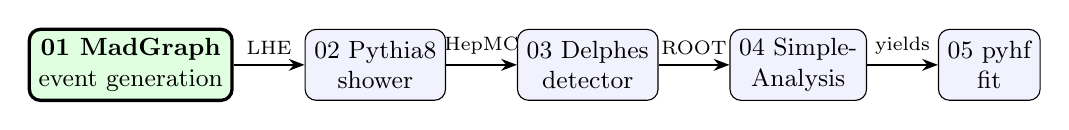
\begin{tikzpicture}[node distance=6mm and 9mm, every node/.style={font=\small},
  box/.style={draw, rounded corners, align=center, minimum height=9mm, fill=blue!5},
  done/.style={draw, rounded corners, align=center, minimum height=9mm, fill=green!12, very thick},
  arr/.style={-{Stealth[length=2mm]}, thick}]
\node[done] (mg) {\textbf{01 MadGraph}\\event generation};
\node[box, right=of mg] (py) {02 Pythia8\\shower};
\node[box, right=of py] (de) {03 Delphes\\detector};
\node[box, right=of de] (sa) {04 Simple-\\Analysis};
\node[box, right=of sa] (hf) {05 pyhf\\fit};
\draw[arr] (mg) -- node[above]{\scriptsize LHE} (py);
\draw[arr] (py) -- node[above]{\scriptsize HepMC} (de);
\draw[arr] (de) -- node[above]{\scriptsize ROOT} (sa);
\draw[arr] (sa) -- node[above]{\scriptsize yields} (hf);
\end{tikzpicture}
\caption{The reinterpretation pipeline. The green box (MadGraph event generation) is the stage
documented here; the arrows are the data files passed between stages.}
\label{fig:pipeline}
\end{figure}

\section{The concrete worked example}
Throughout, the running example is the signal sample at the heart of an ATLAS search for
\emph{sleptons} (defined in Chapter~\ref{ch:physics}). The two input ``cards'' in this stage's
\code{inputs/} directory describe \emph{slepton--pair production} at a specific mass point:
sleptons of mass $200\GeV$ that each decay to a Standard--Model lepton plus an invisible neutralino
of mass $150\GeV$. The parameter card is byte--for--byte identical to the one ATLAS released on
HEPData, so we are reproducing the actual signal simulation that underpins a published result.

% ===========================================================================
\chapter{Physics background, from scratch}
\label{ch:physics}

This chapter builds the minimum physics vocabulary needed to understand what we generate and why.
A reader comfortable with cross--sections and supersymmetry can skim to Chapter~\ref{ch:madgraph}.

\section{Collisions, events, and cross--sections}
At the LHC two beams of protons travel in opposite directions and cross inside detectors. When two
protons (really, their constituent quarks and gluons --- collectively \emph{partons}) interact, we
call the outcome an \textbf{event}: a list of the particles produced and their momenta.

How often does a given kind of event happen? That rate is encoded in a \textbf{cross--section},
$\sigma$, which has units of area. The standard unit is the \emph{barn}; here we use femtobarns,
$1\fb = 10^{-39}\,\text{cm}^2$. The number of events of a given type that an experiment collects is
\begin{equation}
  N \;=\; \sigma \times \mathcal{L},
  \label{eq:nsigma}
\end{equation}
where $\mathcal{L}$ is the \textbf{integrated luminosity} (a measured property of the data set, in
inverse femtobarns). For example, the full LHC ``Run~2'' data set is $\mathcal{L}=140\,\text{fb}^{-1}$;
a process with $\sigma = 50\fb$ therefore yields $N = 50 \times 140 = 7000$ events. Computing
$\sigma$ for a proposed model is exactly what stage~1 does, alongside producing example events.

\begin{quote}\textbf{In one sentence.} The cross--section is the ``how often'' of a process; the
events are simulated examples of ``what it looks like.''\end{quote}

\section{The Standard Model in one page}
The \textbf{Standard Model} (SM) is our current best theory of fundamental particles. It contains:
\emph{quarks} (six kinds: up, down, charm, strange, top, bottom) and \emph{leptons} (electron,
muon, tau, and their neutrinos), which make up matter; and \emph{force carriers} --- the gluon
(strong force), the photon and the $W$/$Z$ bosons (electromagnetic and weak forces), and the Higgs
boson (which gives mass). Protons are bound states of quarks and gluons, which is why a proton
collision is really a collision of those constituents, with a \emph{parton distribution function}
(Chapter~\ref{ch:madgraph}) describing how the proton's momentum is shared among them.

\section{Why go beyond it: supersymmetry}
The SM is incomplete: it has no particle to explain the dark matter that astronomers observe, and
it leaves some theoretical puzzles unresolved. \textbf{Supersymmetry} (SUSY) is a popular extension
that pairs every SM particle with a heavier ``superpartner.'' Superpartners of the leptons are
\textbf{sleptons} ($\slep$); the superpartner mixtures of the neutral bosons include the
\textbf{neutralinos} ($\tilde\chi^0$). In many SUSY models the lightest superpartner is stable and
neutral --- a perfect dark--matter candidate --- called the \textbf{Lightest Supersymmetric
Particle} (LSP). Here the LSP is the lightest neutralino $\neut$.

A stable, neutral LSP does not interact in the detector: it escapes invisibly, carrying away
momentum. Its signature is therefore \textbf{missing transverse momentum} ($E_T^{\text{miss}}$) ---
an apparent imbalance in the momenta we \emph{do} see, in the plane transverse to the beams.

\section{The process we simulate}
Our running example is \textbf{direct slepton--pair production} followed by slepton decay:
\begin{equation}
  p\,p \;\to\; \slep^{+}\,\slep^{-}, \qquad
  \slep^{\pm} \to \ell^{\pm} + \neut .
  \label{eq:process}
\end{equation}
Two protons produce a slepton and an anti--slepton (via an intermediate photon or $Z$ boson); each
slepton decays to its Standard--Model partner lepton ($e$ or $\mu$) plus the invisible $\neut$. The
experimental signature is therefore \textbf{two leptons + missing transverse momentum}.

\paragraph{The mass point ``200/150''.} A \emph{simplified model} fixes just the few masses that
matter and decouples everything else. Ours sets every slepton mass to $200\GeV$ and the neutralino
LSP to $150\GeV$; all coloured superpartners are given an enormous mass ($4.5\times10^{9}\GeV$) so
they never appear. The $50\GeV$ gap between slepton and neutralino is moderately ``compressed'':
the leptons come out fairly soft (low momentum), which is what the ATLAS search was optimised for.
Each slepton is forced to decay to lepton~$+\neut$ with 100\% probability.

\begin{quote}\textbf{In one sentence.} We are producing pairs of 200~GeV sleptons that each turn
into a visible lepton plus an invisible 150~GeV dark--matter--like particle.\end{quote}

% ===========================================================================
\chapter{How MadGraph works}
\label{ch:madgraph}

\textbf{MadGraph5\_aMC@NLO} (hereafter ``MadGraph'') is a \emph{matrix--element event generator}.
This chapter explains what that means, in four conceptual steps. Tutorial slides referenced below
are from the in--workspace deck \emph{tutorial-CMSandATLAS-2016} (M.~Zaro).

\section{Step 1: Feynman diagrams and the matrix element}
Quantum field theory computes the probability \emph{amplitude} for a process as a sum of
\textbf{Feynman diagrams} --- pictorial shorthands for terms in a perturbative expansion. Each
diagram encodes incoming and outgoing particles connected by \emph{propagators} (internal virtual
particles) at \emph{vertices} (interaction points). The sum of all diagrams for a process is its
amplitude $\mathcal{M}$. Probabilities depend on the \emph{squared} amplitude $|\mathcal{M}|^2$.

MadGraph's first job, given a model and a process, is to enumerate every contributing diagram and
write computer code that evaluates $|\mathcal{M}|^2$ for any input momenta. For our example it
generated \textbf{144 subprocesses with 1456 diagrams} (tutorial slides 20--21 show the analogous
output for top--quark pairs).

\section{Step 2: from $|\mathcal{M}|^2$ to a cross--section --- phase--space integration}
The cross--section is obtained by integrating $|\mathcal{M}|^2$ over all the ways the final--state
particles can share the available energy and momentum --- the \textbf{phase space} --- and over the
momentum fractions the colliding partons carry inside the protons. Schematically,
\begin{equation}
  \sigma \;=\; \sum_{a,b}\int \! dx_a\,dx_b\; f_a(x_a,\mu)\,f_b(x_b,\mu)
            \int d\Phi\; |\mathcal{M}_{ab}|^2 ,
  \label{eq:xsec}
\end{equation}
where $f_a(x,\mu)$ is the \textbf{parton distribution function} (PDF) --- the probability of finding
parton $a$ carrying momentum fraction $x$ at energy scale $\mu$ --- and $d\Phi$ is the
phase--space measure. This integral has many dimensions and is done numerically by \textbf{Monte
Carlo integration}: throw random points, evaluate the integrand, average. MadGraph's integrator is
the \emph{MadEvent} component (tutorial slides 14, 58).

\paragraph{PDFs.} We use \code{nn23lo1} (the NNPDF~2.3 leading--order set, LHAPDF id 247000), the
same family ATLAS used. The PDF is built into MadGraph, so no extra software is needed.

\section{Step 3: drawing events --- unweighting}
The Monte Carlo integration naturally produces \emph{weighted} points: each random phase--space
point comes with a probability weight. Real detector data, however, is ``unweighted'' --- every
recorded collision counts once. MadGraph therefore performs \textbf{unweighting}: it keeps or
discards points in proportion to their weight, leaving a sample of equally--weighted events
distributed exactly as nature would produce them. Each surviving event is a list of outgoing
particles and their four--momenta.

\section{Step 4: writing the events --- the LHE file}
The events are written in the \textbf{Les Houches Event} (LHE) format --- a community--standard
text file (here gzip--compressed). It has a header (\code{<init>}) with run metadata and the
cross--section, an embedded copy of the input cards, and one \code{<event>} block per collision.
This file is the deliverable of stage~1; Chapter~\ref{ch:output} dissects it.

\begin{quote}\textbf{In one sentence.} MadGraph turns ``which model, which process'' into ``how
often'' (a cross--section) and ``what it looks like'' (a file of simulated events).\end{quote}

\section{What MadGraph does \emph{not} do here}
At this stage the events are at \textbf{parton level}: the quarks and gluons have not yet been
turned into the sprays of hadrons (``jets'') that a real detector sees, and there is no detector
response. Those are the jobs of Pythia8 and Delphes downstream. MadGraph stops at the LHE file
precisely because we did not install those tools (Chapter~\ref{ch:env}).

% ===========================================================================
\chapter{The three cards}
\label{ch:cards}

MadGraph is steered by three plain--text ``cards'' (tutorial slide 14). Two are provided; the third
is generated automatically and then edited. The agent--track files
\code{agent/checklists/*-decisions.md} give the terse ``what to set'' version; here we explain each.

\section{The process card --- \emph{what} to produce}
The process card is a short script of MadGraph commands. Ours (\code{inputs/proc\_card.dat}) reads,
in essence:
\begin{lstlisting}[style=card]
import model MSSM_SLHA2
define slep = el- el+ er- er+ mul- mul+ mur- mur+
generate     p p > slep slep      $ susystrong @1
add process  p p > slep slep j    $ susystrong @2
add process  p p > slep slep j j  $ susystrong @3
output -f -nojpeg
\end{lstlisting}
Line by line:
\begin{itemize}[nosep]
  \item \code{import model MSSM\_SLHA2} --- load the supersymmetric model (it ships with MadGraph).
  \item \code{define slep = \dots} --- a shorthand for ``any of the left-- or right--handed
        selectrons and smuons.'' Multiparticle labels (tutorial slide 28) let one line stand for many.
  \item \code{generate p p > slep slep} --- produce two sleptons from the proton--proton initial
        state. The \code{\$ susystrong} clause \emph{vetoes} coloured superpartners as
        intermediate states, isolating the pure electroweak production we want.
  \item \code{add process \dots j} and \code{\dots j j} --- also allow one or two extra
        ``jets'' (partons) in the hard process. The \code{@1/@2/@3} tags label the 0--, 1-- and
        2--jet samples so they can be combined consistently later (Chapter~\ref{ch:output}).
  \item \code{output -f -nojpeg} --- write the generated code to disk (\code{-f} overwrites,
        \code{-nojpeg} skips diagram images).
\end{itemize}
The only change we make is to name the output directory on the \code{output} line; this is purely
organisational and is documented in \code{changes/DATA-AND-CARD-CHANGES.md} (change D1).

\section{The parameter card --- the \emph{physics point}}
The parameter card uses the \textbf{SUSY Les Houches Accord} (SLHA) format: blocks of numbers keyed
by each particle's \emph{PDG code} (a standard integer ID). The important blocks for us:
\begin{itemize}[nosep]
  \item \code{Block MASS} --- one line per particle, \code{<PDG> <mass> \# name}. Ours sets PDG
        1000011/2000011 (selectrons) and 1000013/2000013 (smuons) to $200\GeV$, and PDG 1000022
        (the neutralino LSP) to $150\GeV$. Coloured superpartners get $4.5\times10^{9}\GeV$.
  \item \code{DECAY} blocks --- the total width of each particle and its branching ratios. Each
        slepton has a single decay line at 100\% to lepton~$+$~neutralino.
\end{itemize}
The provided card is identical to the ATLAS HEPData release. One technical adjustment was required
to make MadGraph's strict parser accept it; this is the subject of Section~\ref{sec:slha-fix} and
change~D2.

\section{The run card --- \emph{how} to run}
MadGraph writes a sensible default run card when the process is output; we then edit a few fields.
The ones that matter (full rationale in \code{changes/DATA-AND-CARD-CHANGES.md}, change~D3):
\begin{center}\small
\begin{tabular}{@{}lll@{}}
\toprule
Field & Value & Meaning \\
\midrule
\code{ebeam1}, \code{ebeam2} & 6500 & beam energy in GeV (so $\rts=13\TeV$) \\
\code{pdlabel} & \code{nn23lo1} & the PDF set (NNPDF2.3LO) \\
\code{nevents} & 1000 & number of events to generate \\
\code{iseed} & 0 & random seed (0 = new each run) \\
\code{ickkw} & 0 & no MadGraph--side jet matching (see Ch.~\ref{ch:output}) \\
\code{xqcut} & 0 & matching cut (off, since \code{ickkw=0}) \\
\code{ptj} & 20 & minimum jet transverse momentum (GeV) \\
\bottomrule
\end{tabular}
\end{center}

% ===========================================================================
\chapter{The computing environment, and why it matters}
\label{ch:env}

This chapter is for readers who are new to scientific software. It explains every tool we installed
and why. The terse instructions are in \code{agent/steps/02-\dots} and \code{03-\dots}; the formal
change log is \code{changes/ENVIRONMENT-CHANGES.md}.

\section{Why we cannot ``just run it''}
Scientific codes like MadGraph are sensitive to their environment. Three obstacles had to be solved
on the machine used here:
\begin{enumerate}[nosep]
  \item \textbf{No Fortran compiler.} MadGraph's numerical core is written in Fortran and must be
        \emph{compiled} (translated to machine code) before it runs. The machine had no Fortran
        compiler.
  \item \textbf{The wrong Python.} MadGraph~2.9.x is a Python program that uses two modules
        (\code{imp}, \code{distutils}) removed from Python~3.12 onward. The system had Python~3.13,
        which crashes it.
  \item \textbf{No package manager} (no Homebrew/conda) and no administrator rights.
\end{enumerate}

\section{The solution: a self--contained environment}
We installed \textbf{Miniforge}, a minimal distribution of the \code{conda} package manager, into
the project's \code{build/} directory --- no admin rights, nothing system--wide. \code{conda} lets
us create an isolated \textbf{environment} (named \code{mg5}) containing exactly the versions we
need:
\begin{itemize}[nosep]
  \item \textbf{Python 3.10} --- old enough to still have \code{imp}/\code{distutils}.
  \item \textbf{gfortran 13} --- the GNU Fortran compiler, with the macOS SDK wired up so it can
        link executables.
  \item \textbf{make}, and the Python modules \textbf{six} and \textbf{numpy} that MadGraph needs.
\end{itemize}
This environment is regenerable from \code{scripts/00\_\dots} and \code{01\_\dots}, and lives under
\code{build/} (which is git--ignored, because it is large and machine--specific).

\section{The generator itself}
We obtained MadGraph by cloning tag \textbf{v2.9.27} from the official GitHub repository. The
reference paper used v2.9.3, but that exact version is not tagged on GitHub (tags start at v2.9.10).
For a leading--order calculation like ours the patch level does not change the physics; this is
argued in \code{changes/ENVIRONMENT-CHANGES.md} (E3). Four configuration lines were appended to make
runs headless and reproducible (E4).

\begin{quote}\textbf{In one sentence.} \code{conda} gives us a private, correctly--versioned
compiler and Python so MadGraph builds and runs identically on any machine, with no admin
rights.\end{quote}

% ===========================================================================
\chapter{The reproduction, step by step}
\label{ch:repro}

This chapter narrates exactly what happens when the workflow runs, including the errors that arise
on a first attempt and \emph{why} they occur --- which is often where the real understanding lives.

\section{Provisioning (scripts 00--02)}
Running \code{scripts/00\_install\_miniforge.sh} downloads and installs Miniforge; \code{01\_\dots}
creates the \code{mg5} environment and verifies the compiler by building a tiny Fortran ``hello
world'' (a cheap way to retire the single most failure--prone part of the whole workflow);
\code{02\_\dots} clones MadGraph and confirms it launches under Python 3.10.

\paragraph{First real error: the missing \code{six} module.} On the first launch MadGraph stops
with \emph{``madgraph requires the six module.''} \code{six} is a small library that smooths over
Python 2/3 differences; MadGraph imports it at start--up. The fix is one command:
\code{conda install -n mg5 -c conda-forge six numpy}. (Recorded in
\code{agent/checklists/troubleshooting.md}.)

\section{Generating the process code (script 03, part D)}
MadGraph reads the process card and writes the Fortran matrix--element code into
\code{build/runs/slepton\_200\_150/}. Crucially, it also \textbf{auto--generates} the default
\code{run\_card.dat} and \code{param\_card.dat} at this moment --- this is the ``run card generated
at runtime'' that the workflow refers to. The console ends with \emph{``Output to directory \dots
done.''} and reports 144 subprocesses / 1456 diagrams.

\section{Installing the physics inputs (script 03, part E)}
\paragraph{Second real error: \code{InvalidParam}.}\label{sec:slha-fix}
When we replace the default parameter card with the ATLAS one and launch, MadGraph aborts with
\code{InvalidParam} and a Python traceback ending \code{int() \dots 'decay'}. The cause: the ATLAS
card writes twelve Standard--Model decay lines in a non--standard form, e.g.
\begin{lstlisting}[style=card]
DECAY   6    decay 6 1.42E+00  # WT
\end{lstlisting}
The SLHA standard (and MadGraph's parser) expects \code{DECAY 6 1.42E+00}; the extra
\code{decay 6} tokens make the parser try to read the word ``decay'' as an integer. The fix
(\code{scripts/normalize\_param\_card.py}) rewrites \emph{only} those header lines to the standard
form, preserving every width, code, and comment. No mass, mixing, or branching ratio changes ---
and the affected Standard--Model widths do not even enter our matrix element. This is change~D2,
documented at both the workflow and pedagogical levels.

\paragraph{Editing the run card.} The four edits of Chapter~\ref{ch:cards} are applied. Among them,
setting \code{ickkw=0} (and hence \code{xqcut=0}) is the physically meaningful one; the next
section explains why.

\paragraph{Third real warning: \code{xqcut>0 but ickkw=0}.} On a first pass the auto--generated card
had \code{ickkw=1} (turn on MadGraph's own jet matching) with a non--zero \code{xqcut}. Because we
intend to do the matching \emph{later} in the parton shower instead (next chapter), the consistent
choice is \code{ickkw=0} \emph{and} \code{xqcut=0}; otherwise MadGraph warns that the combination is
inconsistent. Setting \code{xqcut=0} removes the warning. This is change~D3.

\section{Generating events (script 03, part F)}
\code{generate\_events} compiles all subprocesses with gfortran, integrates the cross--section,
unweights, and writes the LHE file. A benign message --- \emph{``the width of particle 13
\dots\ too small for an s--channel resonance''} --- refers to the muon's tiny width; the muon is not
an internal resonance in our process, so it is harmless. The run reports
\emph{``Cross--section : \dots pb''} and \emph{``1000 events''}.

% ===========================================================================
\chapter{Reading and validating the output}
\label{ch:output}

A number is only meaningful if you can check it. This chapter shows how to read the LHE file and how
to confirm the result is physically sensible. The terse version is \code{agent/steps/08-\dots}.

\section{Anatomy of the LHE file}
Uncompressing the file and reading the \code{<init>} block reveals the run metadata and the
cross--sections:
\begin{lstlisting}[style=card]
<init>
2212 2212 6.500000e+03 6.500000e+03 0 0 247000 247000 -4 3
4.72e-02 1.4e-04 1.04e-01 1      # 0-jet class:  ~47 fb
2.88e-02 1.7e-04 1.04e-01 2      # 1-jet class:  ~29 fb
2.83e-02 2.9e-04 1.04e-01 3      # 2-jet class:  ~28 fb
</init>
\end{lstlisting}
The first line says: proton (\code{2212}) on proton, each beam $6500\GeV$, PDF id 247000, and three
process classes. The next three lines give each class's cross--section (in picobarns; $1\,\text{pb}=
1000\fb$). Each subsequent \code{<event>} block lists the particles: a status code ($-1$ incoming,
$+1$ outgoing), the PDG id, and the four--momentum. In our sample every event contains exactly one
$\slep^{+}\slep^{-}$ pair, and the slepton lines carry mass $200\GeV$ --- a direct check that the
parameter card took effect.

\section{The cross--section and a sanity check}
For one representative run the inclusive total was $\sigma \approx 104\fb$, split as $\sim$47/29/28
fb across the 0/1/2--jet classes. Is that reasonable? ATLAS quotes (at higher order, NLO+NLL)
$\sigma(\slep_L)=43.9\fb$ and $\sigma(\slep_R)=16.7\fb$, totalling $60.6\fb$. Higher--order
calculations exceed leading order by a ``$k$--factor'' the reference paper measured as 1.18, so the
expected \emph{leading--order} value is $60.6/1.18 \approx 51\fb$. Our \textbf{0--jet (Born)} piece,
$\approx 47\fb$, matches this to about 10\% --- exactly the agreement one expects at leading order.

\section{Why the inclusive total is larger: matching and merging}
\label{sec:merging}
Why is the inclusive total ($104\fb$) about double the Born value ($47\fb$)? Because we generated
the 0--, 1-- and 2--jet matrix elements \emph{separately} and added them. There is overlap between
them: a ``0--jet'' event whose parton later radiates looks like a ``1--jet'' event. Adding the
classes naively \textbf{double--counts} this overlap.

The cure is \textbf{matching/merging}, and there are two schemes (tutorial slides 121, 143--146,
165--173):
\begin{itemize}[nosep]
  \item \textbf{MLM} matching lives inside MadGraph (\code{ickkw=1}, with a cut \code{xqcut}).
  \item \textbf{CKKW--L} merging lives in the parton shower (Pythia8), at a ``merging scale.''
\end{itemize}
The ATLAS sample uses CKKW--L at a merging scale of $m(\slep)/4 = 50\GeV$ --- a step that happens in
\emph{stage~2}, not here. So at this stage we deliberately set \code{ickkw=0}: MadGraph emits the
raw, overlapping multi--jet sample, and the downstream shower removes the double counting. The
honest, comparable number from stage~1 alone is therefore the Born (0--jet) piece, which is why our
sanity check used it. The extra--jet generation cut \code{ptj=20} (kept below the $50\GeV$ merging
scale) regularises the otherwise--divergent extra--jet rates.

\begin{quote}\textbf{In one sentence.} The inclusive total double--counts on purpose; the parton
shower (stage~2) will merge the samples, and until then the Born piece is the trustworthy
number.\end{quote}

\section{The event content}
A quick tally of the 1000 events shows the jet multiplicities split roughly 45/27/27\% (0/1/2 jets),
matching the cross--section fractions as it must for unweighted events. Left-- and right--handed
sleptons appear in about a 70:30 ratio, mirroring the ATLAS $\sigma(\slep_L):\sigma(\slep_R)$ ratio.
These internal consistencies are themselves validation.

% ===========================================================================
\chapter{Generalising the workflow}
\label{ch:general}

The point of the project is not this one sample but a \emph{repeatable process}. The agent track is
written to be general; here is the decision logic a human (or agent) follows for a \emph{new}
request, mirroring \code{agent/checklists/}.

\paragraph{1. What process?} Translate the request into \code{generate}/\code{add process} lines:
choose the model, the final state, whether to include extra jets, and which intermediate states to
veto. (\code{checklists/process-card-decisions.md}.)

\paragraph{2. What physics point?} Edit the \code{Block MASS} entries for the relevant PDG codes and
set the decays; decouple anything that should not appear. Normalise the SLHA card if MadGraph
rejects it. (\code{checklists/parameter-card-decisions.md}.)

\paragraph{3. How to run?} Set $\rts$ via \code{ebeam}, the event count, the seed, and --- if the
process has multiple jet multiplicities --- the matching choice. For shower--side (CKKW--L) merging
use \code{ickkw=0}; for self--contained MLM use \code{ickkw=1} with an \code{xqcut}.
(\code{checklists/run-card-decisions.md}.)

\paragraph{4. Check in.} Confirm the process card and the key run settings with the scientist before
a long run; incorporate feedback by revisiting only the affected step. (\code{shared/agent/ORCHESTRATION.md}.)

The same scripts work for any leading--order process; only the cards and a few run--card fields
change. A different mass point reuses the already--compiled process directory and only re--runs the
integration.

% ===========================================================================
\chapter{Limitations and what comes next}
\label{ch:limits}

\begin{itemize}[nosep]
  \item \textbf{Parton level only.} The output has no parton shower, hadronisation, or detector
        effects. It is an \emph{input} to those stages, not a physics result on its own.
  \item \textbf{Leading order.} Cross--sections are LO; a $k$--factor (here 1.18) is applied
        downstream to approximate higher orders.
  \item \textbf{No merging yet.} The inclusive multi--jet total double--counts until the stage--2
        shower merges it (Section~\ref{sec:merging}).
  \item \textbf{Version.} v2.9.27, not the paper's v2.9.3 (unavailable on GitHub); immaterial at LO.
  \item \textbf{Statistics.} The example uses 1000 events for speed; production samples use far more
        (the paper used 50000). Raise \code{nevents} and enable multi--core running for those.
\end{itemize}
The next stage (Pythia8) consumes this LHE file, showers and hadronises it, and performs the CKKW--L
merging; see \code{../../../shared/agent/ORCHESTRATION.md}.

% ===========================================================================
\appendix
\chapter{Glossary}
\begin{description}[style=nextline,leftmargin=0pt,font=\bfseries\ttfamily]
  \item[cross--section ($\sigma$)] interaction rate, in units of area; events $=\sigma\times\mathcal{L}$.
  \item[luminosity ($\mathcal{L}$)] a measure of how much data was collected, in $\text{fb}^{-1}$.
  \item[event] one simulated (or real) collision: a list of particles and momenta.
  \item[matrix element] the quantum amplitude $\mathcal{M}$; $|\mathcal{M}|^2$ drives probabilities.
  \item[phase space] the set of allowed final--state momentum configurations.
  \item[PDF] parton distribution function; the momentum content of the proton.
  \item[LHE] Les Houches Event format; the parton--level event file MadGraph writes.
  \item[parton level] before the shower turns quarks/gluons into jets of hadrons.
  \item[LO / Born] leading order; the lowest--order (here 0--jet) contribution.
  \item[$k$--factor] ratio of a higher--order to the LO cross--section.
  \item[MLM / CKKW--L] two schemes for combining matrix--element multiplicities with the shower
        without double counting.
  \item[SLHA] SUSY Les Houches Accord; the parameter--card text format.
  \item[LSP / $\neut$] lightest supersymmetric particle; stable, invisible $\Rightarrow$ missing momentum.
  \item[slepton ($\slep$)] scalar superpartner of a lepton.
  \item[PDG code] standard integer identifier for each particle.
\end{description}

\chapter{Reproducing this run end to end}
From the stage directory (\code{stages/01-event-generation/}):
\begin{lstlisting}
bash scripts/00_install_miniforge.sh
bash scripts/01_create_env.sh
build/tools/miniforge3/bin/conda install -y -n mg5 -c conda-forge six numpy
bash scripts/02_get_madgraph.sh
NEVENTS=1000 bash scripts/03_run_madgraph.sh run_02
\end{lstlisting}
Output: \code{build/runs/slepton\_200\_150/Events/run\_02/unweighted\_events.lhe.gz}.

\chapter{References}
\begin{enumerate}[nosep]
  \item G.~Stark, C.~Aristimuno Ots, M.~Hance, \emph{Reduce, Reuse, Reinterpret: an end-to-end
        pipeline for recycling particle physics results}, arXiv:2306.11055.
  \item J.~Alwall \emph{et al.}, \emph{The automated computation of tree-level and next-to-leading
        order differential cross sections, and their matching to parton shower simulations},
        JHEP 07 (2014) 079 (MadGraph5\_aMC@NLO).
  \item M.~Zaro, \emph{MadGraph5\_aMC@NLO tutorial} (CMS \& ATLAS, 2016) --- the slide deck in this
        workspace.
  \item ATLAS Collaboration, \emph{Searches for electroweak production of supersymmetric particles
        with compressed mass spectra in $\rts=13\TeV$ pp collisions}, Phys.\ Rev.\ D 101 (2020)
        052005, and its HEPData record.
  \item The agent track of this stage (\code{agent/WORKFLOW.md}) and the change registry
        (\code{changes/}).
\end{enumerate}

\end{document}
